\documentclass[12pt]{article}
\usepackage{fancyhdr}
\pagestyle{fancy}
\fancyhf{}
\fancyfoot[C]{\thepage}
\fancyfoot[L]{\scriptsize CC BY-NC-SA 4.0 \textbullet\ Leo Liang}
\renewcommand{\headrulewidth}{0pt}
\usepackage[margin=1in]{geometry}
\usepackage{amsmath, amssymb}
\usepackage{array, booktabs}
\usepackage{pgffor}
\usepackage{tikz}
\parindent=0pt
\parskip=1em
\newcolumntype{C}[1]{>{\centering\arraybackslash}p{#1}}
\newcommand{\wl}{\par\vspace{5mm}\noindent\rule{\linewidth}{0.4pt}\par\vspace{1mm}}
\newcommand{\wls}[1]{\foreach \i in {1,...,#1}{\wl}}
\newcommand{\gridaxes}[1]{%
  \draw[step=1,gray!25,very thin] (-#1,-#1) grid (#1,#1);%
  \draw[thick,->] (-#1-0.4,0)--(#1+0.4,0) node[right]{$x$};%
  \draw[thick,->] (0,-#1-0.4)--(0,#1+0.4) node[above]{$y$};%
  \foreach \n in {-#1,...,#1}{\ifnum\n=0\else
      \draw (\n,0.08)--(\n,-0.08) node[below]{\scriptsize$\n$};
      \draw (0.08,\n)--(-0.08,\n) node[left]{\scriptsize$\n$};\fi}%
}
% ─────────────────────────────────────────────────────────────────────────────
\begin{document}
\pagestyle{fancy}
\begin{center}
  {\Large\bfseries Homework 7}\\[4pt]
  Domain \& Range Practice, and an Introduction to Limits\\[6pt]
  Name:\;\underline{\hspace{6.5cm}}\quad
\end{center}
\hrule\bigskip

\section*{Instructions}
Use a \textbf{pen} and \textbf{show every step}. Part 1 is more practice with the domain-and-range method from last
time --- the goal is to make the procedure automatic. Part 2 introduces \textbf{limits} from three angles. Write
questions in the margin in a different color. You may use AI as a \textbf{teacher}, but try each problem yourself first. 

Some questions in part 2 may be unfamiliar to you. You should ask AI to teach you those concepts.

% ===========================================================================
\section*{Part 1 --- Domain and Range (more practice)}
Refer to the reading from homework 6 on how to write a detailed response. You should imitate that structure for the following problems.

\textit{Method reminder.}\quad For the \textbf{domain}, avoid the two dangers: no dividing by zero, and no square
roots of negatives. For the \textbf{range}, set $y = f(x)$ and \textbf{solve for $x$}; the range is the set of
$y$-values that give a valid $x$. 

The first problem will begin on the next page.

\newpage
\textbf{1.}\quad $f(x) = \sqrt{x - 4}$.\quad Find the domain and range.

\newpage

\bigskip
\textbf{2.}\quad $g(x) = \dfrac{3x}{\,x + 1\,}$.\quad Find the domain and range.

\newpage
\textbf{3.}\quad $h(x) = x^2 - 5$.\quad Find the domain and range.


% ===========================================================================
\newpage
\section*{Part 2 --- Introduction to Limits}
A \textbf{limit} asks: as $x$ gets close to a number $a$, what value is $f(x)$ heading toward? We write
\[
  \lim_{x \to a} f(x).
\]
The limit is about where $f$ is \emph{headed} as $x$ approaches $a$ --- not its value \emph{at} $a$, which may be
different, or may not even exist. Below you will find a limit three ways: from a \textbf{graph}, from a
\textbf{table}, and with \textbf{algebra}.

\subsection*{Angle 1 --- Read the limit from a graph}

\textbf{4.}\quad Use the graph of $f$ below.

\begin{center}
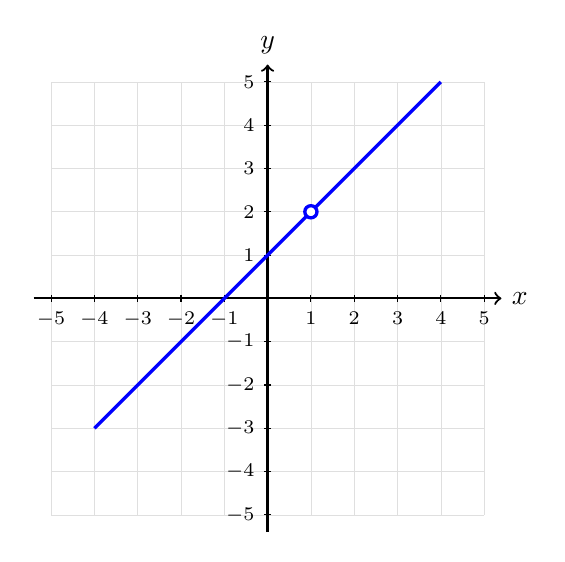
\begin{tikzpicture}[scale=0.55]
  \gridaxes{5}
  \draw[very thick, blue] (-4,-3)--(4,5);
  \fill[white] (1,2) circle (4pt);
  \draw[very thick, blue] (1,2) circle (4pt);
\end{tikzpicture}
\end{center}

\textbf{(a)}\quad $\displaystyle\lim_{x \to 1} f(x) = \underline{\hspace{2.5cm}}$

\medskip
\textbf{(b)}\quad Is $f(1)$ defined? How can you tell from the graph?
\wl

\newpage
\bigskip
\textbf{5.}\quad Use the graph of $g$ below.

\begin{center}
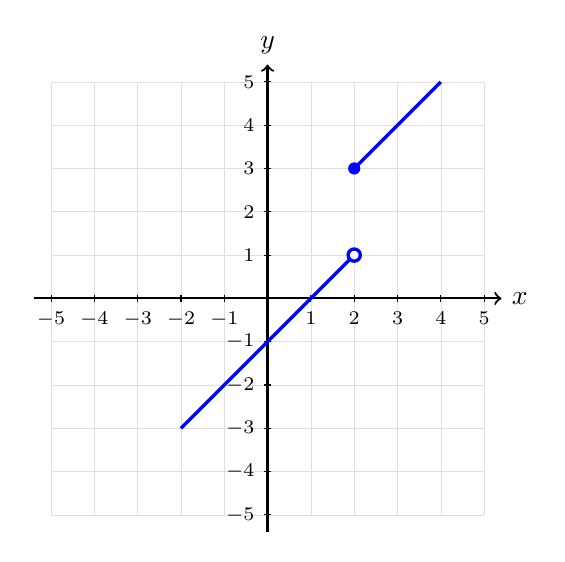
\begin{tikzpicture}[scale=0.55]
  \gridaxes{5}
  \draw[very thick, blue] (-2,-3)--(2,1);
  \fill[white] (2,1) circle (4pt);
  \draw[very thick, blue] (2,1) circle (4pt);
  \draw[very thick, blue] (2,3)--(4,5);
  \fill[blue] (2,3) circle (4pt);
\end{tikzpicture}
\end{center}

\textbf{(a)}\quad Approaching $x = 2$ from the \textbf{left}, $g(x) \to \underline{\hspace{2cm}}$\qquad

\textbf{(b)}\quad From the \textbf{right}, $g(x) \to \underline{\hspace{2cm}}$

\medskip
\textbf{(c)}\quad Does $\displaystyle\lim_{x \to 2} g(x)$ exist? Explain.
\wl

\textbf{(d)}\quad $g(2) = \underline{\hspace{2cm}}$

\subsection*{Angle 2 --- Read the limit from a table}

\textbf{6.}\quad The table shows values of $f(x) = \dfrac{x^2 - 9}{\,x - 3\,}$ near $x = 3$. (Note: $f(3)$ is
$\tfrac{0}{0}$, undefined.) What does $\displaystyle\lim_{x \to 3} f(x)$ appear to be?

\medskip
\renewcommand{\arraystretch}{1.4}
\begin{tabular}{|C{1.6cm}|C{1.4cm}|C{1.4cm}|C{1.6cm}|C{1.6cm}|C{1.4cm}|C{1.4cm}|}
\hline
$x$ & $2.9$ & $2.99$ & $2.999$ & $3.001$ & $3.01$ & $3.1$ \\
\hline
$f(x)$ & $5.9$ & $5.99$ & $5.999$ & $6.001$ & $6.01$ & $6.1$ \\
\hline
\end{tabular}
\renewcommand{\arraystretch}{1}

\medskip
$\displaystyle\lim_{x \to 3} f(x) = \underline{\hspace{2.5cm}}$


\newpage
\textbf{7.}\quad The table shows values of $h(x)$ near $x = 1$.

\medskip
\renewcommand{\arraystretch}{1.4}
\begin{tabular}{|C{1.6cm}|C{1.4cm}|C{1.4cm}|C{1.6cm}|C{1.6cm}|C{1.4cm}|C{1.4cm}|}
\hline
$x$ & $0.9$ & $0.99$ & $0.999$ & $1.001$ & $1.01$ & $1.1$ \\
\hline
$h(x)$ & $1.9$ & $1.99$ & $1.999$ & $4.001$ & $4.01$ & $4.1$ \\
\hline
\end{tabular}
\renewcommand{\arraystretch}{1}

\medskip
(a) Approaching from the left, $h(x) \to \underline{\hspace{2cm}}$;\quad 

(b) From the right, $h(x) \to
\underline{\hspace{2cm}}$.\quad 

(c) Does $\displaystyle\lim_{x \to 1} h(x)$ exist? Explain.
\wl

\subsection*{Angle 3 --- Find the limit with algebra}
\textit{First try substituting the number for $x$. If you get an ordinary number, that is the limit. If you get
$\tfrac{0}{0}$, factor the top and bottom, cancel, and then substitute.}

\medskip
\textbf{8.}\quad Find each limit. Show your steps.

\medskip
\textbf{(a)}\quad $\displaystyle\lim_{x \to 4} (3x - 5)$

\vspace{9em}

\textbf{(b)}\quad $\displaystyle\lim_{x \to 2} (x^2 + x - 1)$

\newpage
\textbf{(c)}\quad $\displaystyle\lim_{x \to 1} \frac{x^2 - 1}{\,x - 1\,}$

\vspace{22em}

\textbf{(d)}\quad $\displaystyle\lim_{x \to 3} \frac{x^2 - 9}{\,x - 3\,}$ \quad (compare with your answer to Q6!)


\newpage

\textbf{(e)}\quad $\displaystyle\lim_{x \to 2} \frac{x^2 - 4}{\,x^2 - x - 2\,}$

% ===========================================================================
\newpage
\section*{Notebook Artifact}

\bigskip
\textbf{N1.}\quad If you used the internet or AI, describe how you used it.
\wls{4}

\end{document}